\section{Analysis of the MPJPE when deviating from the constraints}

Possible deviations of the assumptions about the three dimensional poses and how they are projected onto the image plane: Deviation in x and y direction, deviation in z direction, different focal length.

We regard the system as a black box that takes a normalized set of two dimensional points as input and outputs the depths (the z coordinates) of the input points which then can be reprojected into three dimensional space.
\subsection{Shifting along one image plane axis}
\Todo{Add introduction to nomenclature and notation.}
\label{sec:x-shift-error}
\subsubsection{Theoretical analysis}
\Todo{Properly define the pose and the camera.}
Let $P_i=(x_i, y_i, z_i) \in \mathbb{R}^3$ and $f$ the focal length of a camera which is located at the origin along the x-y-plane and looks at $(0, 0, z)$, the location of the root joint. 
Assume $P_i$ is shifted by $dx$ along the x axis.
The x coordinate of the projected point on the image plane is
\begin{equation}
	x_i^\mathrm{P} = f \frac{x_i + dx}{z_i} = f \frac{x_i}{z_i} + f \frac{dx}{z_i}\ .
\end{equation}
Subsequently all projected points are shifted along the x axis such that the root node which is located at $(0, 0, z)$ is in the origin of the image plane. That means:
\begin{equation}
	\widetilde{x}_i^\mathrm{P} = f \frac{x_i}{z_i} + f \frac{dx}{z_i} - f \frac{dx}{z} 
	= f \frac{x_i}{z_i} + f dx (\frac{1}{z_i} - \frac{1}{z})
	= x_i^\mathrm{P} + f dx (\frac{1}{z_i} - \frac{1}{z})\ .
\end{equation}
After the system estimated the depth $\widetilde{z}_i$ of the point, it is reprojected into three dimensions. The resulting x coordinate is 
\begin{equation}
	\widetilde{x}_i^\mathrm{R} = \frac{\widetilde{x}_i^\mathrm{P}}{f} \cdot \widetilde{z}_i
	= x_i \frac{\widetilde{z}_i}{z_i} + dx (\frac{1}{z_i} - \frac{1}{z}) \widetilde{z}_i
\end{equation}
The euclidean distance of the reprojected point to the original point is given by
\begin{equation}
\label{eq:delta-d}
	\Delta d_i = \norm{ 
	\begin{pmatrix}
		\widetilde{x}_i^R - x_i \\
		\widetilde{z}_i - z_i
	\end{pmatrix}
	}_2
\end{equation}
This expression takes on its minimum when 
\begin{equation}
	\label{eq:minimum-distance}
	f(\widetilde{z}_i) = \left ( \widetilde{z}_i \cdot \left( \frac{x_i}{z_i} + dx \left( \frac{1}{z_i} - \frac{1}{z} \right) \right ) - x_i \right)^2 + ( \widetilde{z}_i - z_i ) ^2
\end{equation}
is minimal. 
Substituting $a = \left( \frac{x_i}{z_i} + dx \left( \frac{1}{z_i} - \frac{1}{z} \right) \right )$ makes the equation more readable. 
In order to obtain the optimal value for $\widetilde{z}_i$, \eqref{eq:minimum-distance} is differentiated by $\widetilde{z}_i$:
\begin{equation}
	f'(\widetilde{z}_i) = 2 \cdot (\widetilde{z}_i a^2 - a x_i + \widetilde{z}_i - z_i)
\end{equation}
Setting this equal to zero gives
\begin{align*}
	0 &= f'(\widetilde{z}_i) \\
	\Leftrightarrow \widetilde{z}_i & = \frac{a x_i + z_i}{1 + a^2} \ .
\end{align*}
Substituting this into \eqref{eq:delta-d} again yields a total minimal error of 
\begin{equation}
	\label{eq:minimum-delta-d}
	\Delta d_i = \sqrt{\frac{(a z_i - x_i)^2}{a^2 + 1}}\
	= dx (1 -  \frac{z_i}{z}) \sqrt{\frac{1}{a^2 + 1}} .
\end{equation}
The MPJPE $\Delta d$ for a pose can then be calculated as the mean of all $\Delta d_i$s.

\subsubsection{Experimental results}
	In practice, the observable error has the same approximate shape of this function, but is much smaller than the theoretical results.
	The reason for this is the scaling that is applied to the inferred poses during the evaluation of Protocol 2 (section \ref{sec:protocol2}).
	\unsure{Validate if this is really the case. Also see in what way it is proportional.}
	It appears that the average limb length of the inferred shifted poses is increasing monotonously with increasing offset $dx$.
	That means the poses are downsized by a factor $\alpha$ in all dimensions. 
	\Todo{Explain why} Therefore the actual error is $\Delta d' = \alpha \cdot \Delta d$.
	
	\begin{figure}[ht]
		
		\centering
		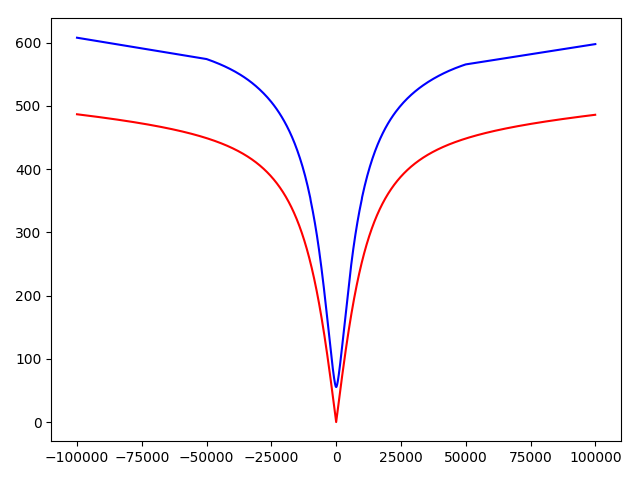
\includegraphics[scale=0.5]{images/x_shift_error.png}
		\caption{Plot of theoretical (red) and observed (blue) MPJPEs for different values of $dx$. 
			The theoretical errors are obtained by calculating the mean of the per pose errors $\alpha \Delta d$ for the evaluation data.}
		\Todo[inline]{Add axes titles, use proper image.
		use pgfplots to plot data}
		\label{fig:x-shift-error}
	\end{figure}

	It is noticeable that the performance of the network is not worse than the theoretical results by a constant offset.
	For small deviations along the x axis the network seems to be able to compensate the error introduced by shifting.
	As $dx$ increases, so does the offset between the observed and the theoretical results until it seems to converge to a constant.
	This motivates adjusting not only how the inferred points are reprojected into three dimensions but also the input the network receives.
	This will be discussed further in section \ref{sec:network-adjusting}.
	
	As shown in section \ref{sec:data-results} the MPJPE for the original 2D poses is about \Todo{Check this number} 30mm higher than the one for the synthetically generated data.
	The simplest explanation for this is that the original 2D poses do not fulfill the constraints for the system.
	The camera is not centered on the root joint and also the camera distance is most certainly not exactly ten times the length of the norm limb.
	
	Numbers: ...
	
\subsection{Shifting along the z axis}
\label{sec:z-shift-error}
\subsubsection{Theoretical analysis}
Again consider a point $P_i=(X_i, Y_i, Z_i) \in \mathbb{R}^3$. Assume that $P_i$ is shifted by $dz$ along the z axis.
The x coordinate of the projected point on the image plane is
\begin{equation}
	x_i = f \frac{X_i}{Z_i + dz}
\end{equation}
The projected points are now scaled in a way that they have the same (arbitrary) scale.  Let $\alpha$ be the scale of the set of the original projected points and $\beta$ the one of the set of shifted projected points. The scaled projected point is given by

\begin{equation}
		\widetilde{x}_i = x_i \cdot \frac{\alpha}{\beta} 
		= f \frac{Z_i}{Z_i + dz}\cdot \frac{\alpha}{\beta} 
\end{equation}
After the system estimates the depth $\widetilde{Z}_i$ of each point, they are reprojected into 3 dimensional space.
The reprojected points are given by
\begin{equation}
	\widetilde{X}_i = \frac{\widetilde{x}_i}{f} \cdot \widetilde{Z}_i
	= \frac{X_i}{Z_i + dz}\cdot \frac{\alpha}{\beta}  \cdot \widetilde{Z}_i
\end{equation}
Again we want to minimize equation \eqref{eq:delta-d}.
If we define $a := \frac{X_i}{Z_i + dz}\cdot \frac{\alpha}{\beta}$, the minimal value for $\Delta d$ is the same as in equation \eqref{eq:minimum-delta-d}.


\subsubsection{Experimental results}
	This phenomenon is also affecting our ground truth data. The poses are all projected with a camera distance $ \text{length-of-norm-limb} \cdot 10$. 
	That means the length of the projected norm limb is not exactly $0.1$ but a bit smaller or bigger. 
	Like in the discussed above those projected poses are then normalized. 
	The system estimates the depths of the normalized pose and re-projects it assuming a perfect perspective projection. 
	It therefore does not consider the effect of small deviations in z direction.
	A way to fix this would be to calculate the perfect camera distance for each pose individually before projecting them onto the image plane.
	This is not very realistic though since one might be able to determine the camera's distance to a human approximately, but definitely not exactly. This phenomenon therefore is kind of inevitable.
 
	
\subsection{Total minimal error}

Combining results of the previous two chapters

\subsection{Alternation of the focal length}
No difference

